% Created 2018-01-14 Sun 21:38
\documentclass[bigger]{beamer}
\usepackage[utf8]{inputenc}
\usepackage[T1]{fontenc}
\usepackage{fixltx2e}
\usepackage{graphicx}
\usepackage{grffile}
\usepackage{longtable}
\usepackage{wrapfig}
\usepackage{rotating}
\usepackage[normalem]{ulem}
\usepackage{amsmath}
\usepackage{textcomp}
\usepackage{amssymb}
\usepackage{capt-of}
\usepackage{hyperref}
\usetheme{default}
\author{Alex, Yongki Kim}
\date{01.23.2017}
\title{Simple Git Tutorial}
\hypersetup{
 pdfauthor={Alex, Yongki Kim},
 pdftitle={Simple Git Tutorial},
 pdfkeywords={},
 pdfsubject={Using emacs org-mode, write git manual},
 pdfcreator={Emacs 25.3.1 (Org mode 8.3.4)}, 
 pdflang={English}}
\begin{document}

\maketitle
\begin{frame}{Outline}
\tableofcontents
\end{frame}


\section{Preface}
\label{sec:orgheadline1}
presentation mode: \href{./git_usage_20180113.html}{Git Usage}

\rule{\linewidth}{0.5pt}

This article shows you how to create simple git server and explain how to use git command.
for example, git clone, add, commit, push. 
most important thins is to understand the git's concept and basic terminology, if not, it's not easy to soak into git world.

\section{Git Concept}
\label{sec:orgheadline1}
\subsection{Basic Terminology}
\label{sec:orgheadline1}
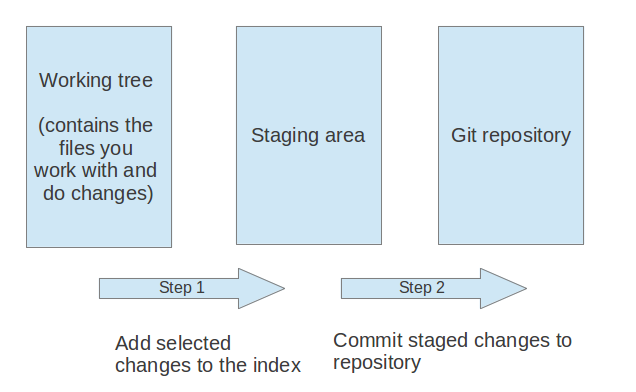
\includegraphics[width=.9\linewidth]{./git-term.png}

\begin{center}
\begin{tabular}{ll}
working tree & the set of working files for the repository. these files are changed and committed to repository.\\
stage(or index) & the place to store changes in the working tree before the commit.\\
repository & origin: normally indicate remote repository\\
branch & a named pointer to a commit, \alert{master} is default.\\
 & master: normall your own branch\\
 & check out: selecting a branch\\
tag & a commit which uniquely identifies a version of the Git repository.\\
pull request & proposing your changes and requesting that someone review and pull in your contribution and merge them into their branch\\
\end{tabular}
\end{center}


\begin{quote}
for more detailed explaination, please refer to \url{http://www.vogella.com/tutorials/Git/article.html}
\end{quote}


\subsection{Git Operation}
\label{sec:orgheadline1}
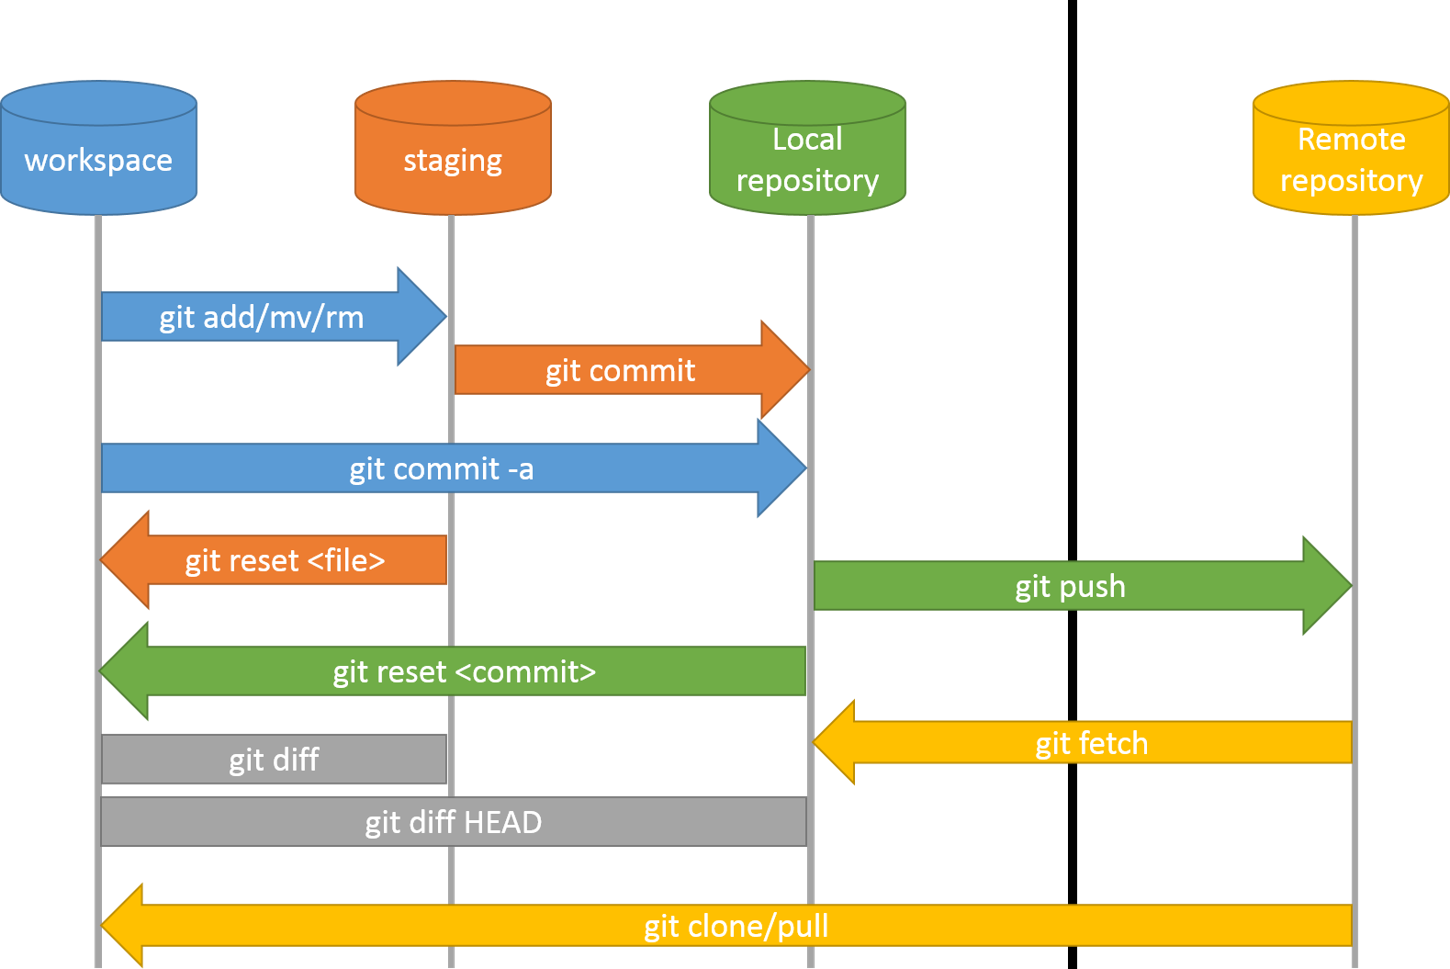
\includegraphics[width=.9\linewidth]{./git-operations.png}

\section{SSH Setting for Git}
\label{sec:orgheadline1}
remember just one thing. 
Private is on client and public key is on server.
\subsection{Necessary Command}
\label{sec:orgheadline1}
\begin{itemize}
\item generating ssh key: ssh-keygen -f \textasciitilde{}/.ssh/git.priv
\item copy ssh public key: cat git.priv | ssh git@server "cat >> .ssh/authorized\(_{\text{keys}}\)"
\item ssh-add \textasciitilde{}/.ssh/git.priv
\end{itemize}

\section{Setting up private git repository}
\label{sec:orgheadline1}
Sometimes you should create your own git repository, but github, specially in closed network environment.
So the first section is to make your own git repository.
\begin{itemize}
\item ref: \url{https://git-scm.com/book/en/v2/Git-on-the-Server-Setting-Up-the-Server}
\end{itemize}

\subsection{demo environment}
\label{sec:orgheadline1}
To make you understand easily, I assume below demo environment.
  \alert{* demo environment *}
\begin{itemize}
\item git server: vm1
\item git client computer: vm2
\item developer1: John on vm2
\item developer2: Jane on vm2
\end{itemize}

\subsection{git user on git server}
\label{sec:orgheadline1}
At first, we will create git user to allow other user's connection.
\begin{quote}
Original guide lets user create ssh-key, but I'll just use password type on ssh connection.
It is better to use ssh-key, but I want to keep focus on the git based command.  
\end{quote}

\#+BEGIN\(_{\text{SRC}}\) 
\#\# on git server
vm1\(sudo adduser git
vm1\) sudo passwd git
vm1\$ su git
\#+END\(_{\text{SRC}}\) shell

\subsection{make git repository on git server}
\label{sec:orgheadline1}
Let's create \alert{project} directory and initialize it.

\#+BEGIN\(_{\text{SRC}}\) shell 
\#\# on git server
vm1\(mkdir ~git/test_project.git
vm1\) cd \textasciitilde{}git/test\(_{\text{project.git}}\)
vm1\$ git init --bare
Initialized empty Git repository in \emph{home/git/test\(_{\text{project.git}}\)} \#\# <-- remember this path, copy it. 
\#+END\(_{\text{SRC}}\) shell

\subsection{Create John's project named 'test\(_{\text{project}}\)'}
\label{sec:orgheadline1}
John will create the 1st project.

\#+BEGIN\(_{\text{SRC}}\) shell 
\#\# as John user on vm2
john@vm2\(mkdir myproject
john@vm2\) cd myproject
john@vm2\(git init
john@vm2\) echo "the first released project" > README.md
john@vm2\(git add .
john@vm2\) git commit -m 'the 1st'
john@vm2\(git remote add origin git@vm1:/home/git/test_project.git ## <-- paste it from above
john@vm2\) git push origin master
\#+END\(_{\text{SRC}}\) shell

You will get some \uline{password} message for ssh-key after \alert{* git push origin master *} command.
Then, press \alert{ENTER} and you will be asked 'ssh password', at this time, input \alert{git's password}.
\subsection{Clone 'test\(_{\text{project}}\)' for Jane}
\label{sec:orgheadline1}

Jane will modify the file and push to master.

\#+BEGIN\(_{\text{SRC}}\) shell 
\#\# as Jane user on vm2
jane@vm2\(git clone git@vm1:/home/git/test_project.git
jane@vm2\) cd test\(_{\text{project}}\)
jane@vm2\(echo "jane's code is add here" >> README.md
jane@vm2\) git add README.md
jane@vm2\(git commit -m 'new code added by jane'
jane@vm2\) git push origin master
\#+END\(_{\text{SRC}}\) shell


\section{Basic Git Usage}
\label{sec:orgheadline1}
\begin{itemize}
\item ref: kor: \url{https://backlog.com/git-tutorial/kr/intro/intro1_2.html}
\item ref: en: \url{http://rogerdudler.github.io/git-guide/}
\end{itemize}
\subsection{Online Git Practice}
\label{sec:orgheadline1}
just follow the below sandbox, this is better than I can explain
\begin{itemize}
\item \url{https://try.github.io/levels/1/challenges/1}
\end{itemize}


\section{Git Workflow}
\label{sec:orgheadline1}
\subsection{Workflow Diagram}
\label{sec:orgheadline1}
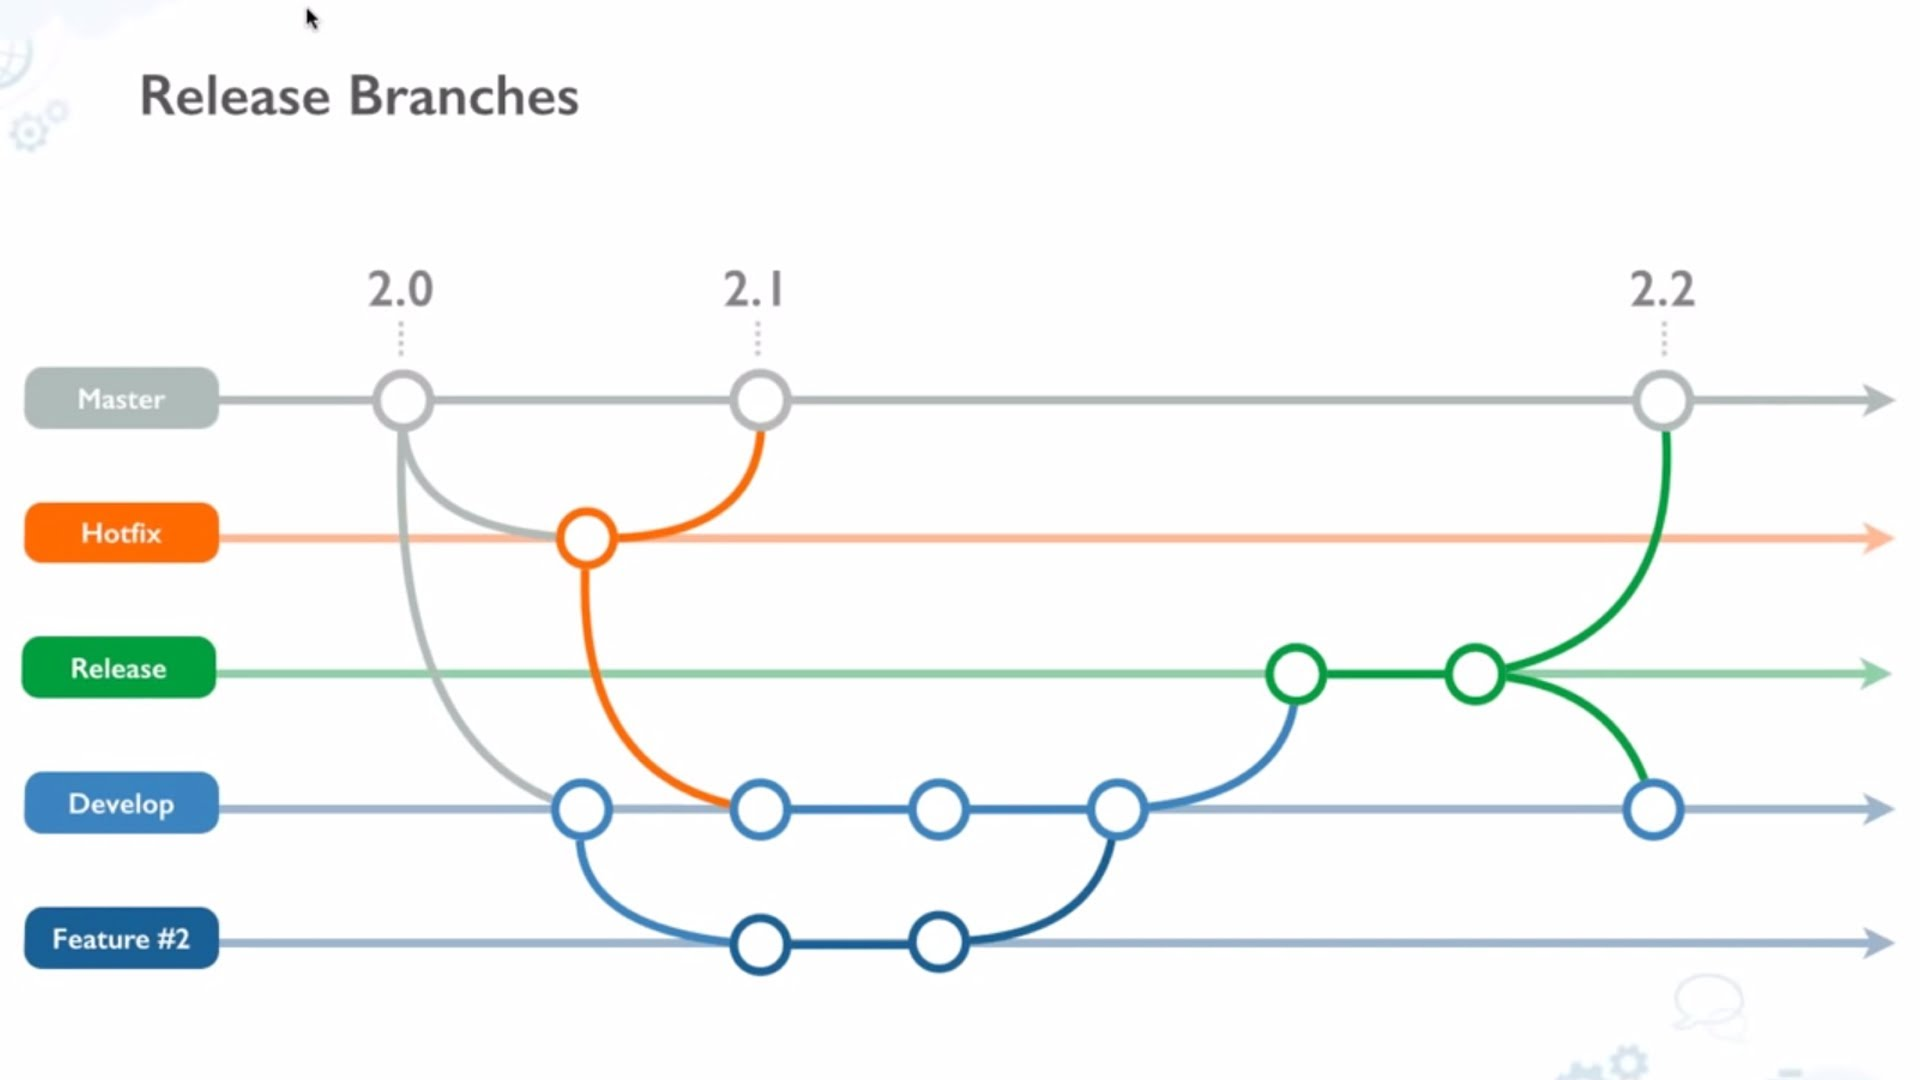
\includegraphics[width=.9\linewidth]{./git-workflow.jpg}

\begin{itemize}
\item ref: \url{https://guides.github.com/activities/hello-world/}
\end{itemize}

\#+BEGIN\(_{\text{SRC}}\) shell 

\#+END\(_{\text{SRC}}\) shell

\section{Conclution}
\label{sec:orgheadline1}
Git is very useful to manage your contents not only source codes but also your own documents. 
Also in this devops erra, knowing the git workflow makes you communicate with other organization easily.
I hope this document to be helpful.
\end{document}
